\documentclass[10pt]{beamer}

\usetheme[progressbar=frametitle]{metropolis}
\usepackage{appendixnumberbeamer}
\usepackage{pgf}
\usepackage{units}
\usepackage{graphicx}
\usepackage{caption}
\usepackage[mode=buildnew]{standalone}% requires -shell-escape
\usepackage{amsmath}

\usepackage[english]{babel}
\usepackage[utf8x]{inputenc}
\setbeamertemplate{footline}[frame number]

\title{Building an end-to-end speech recognizer}
\author{Moritz Wolter}

\date{01.02.2017}


\begin{document}
\begin{frame}
  \titlepage
\end{frame}


% Uncomment these lines for an automatically generated outline.
\begin{frame}{Outline}
  \tableofcontents
\end{frame}

\section{Introduction}
\begin{frame}{The problem}
	\begin{itemize}
		\item What is being said?
		\item How is the data aligned?
		\item What model architecture?
		\item What are good hyper-parameters?
		\item How to ensure generalization?
	\end{itemize}
\end{frame}

\begin{frame}{The LAS-Architecture}
	\begin{figure}
		\begin{tikzpicture}
		    \node[anchor=south west,inner sep=0] at (0,0) {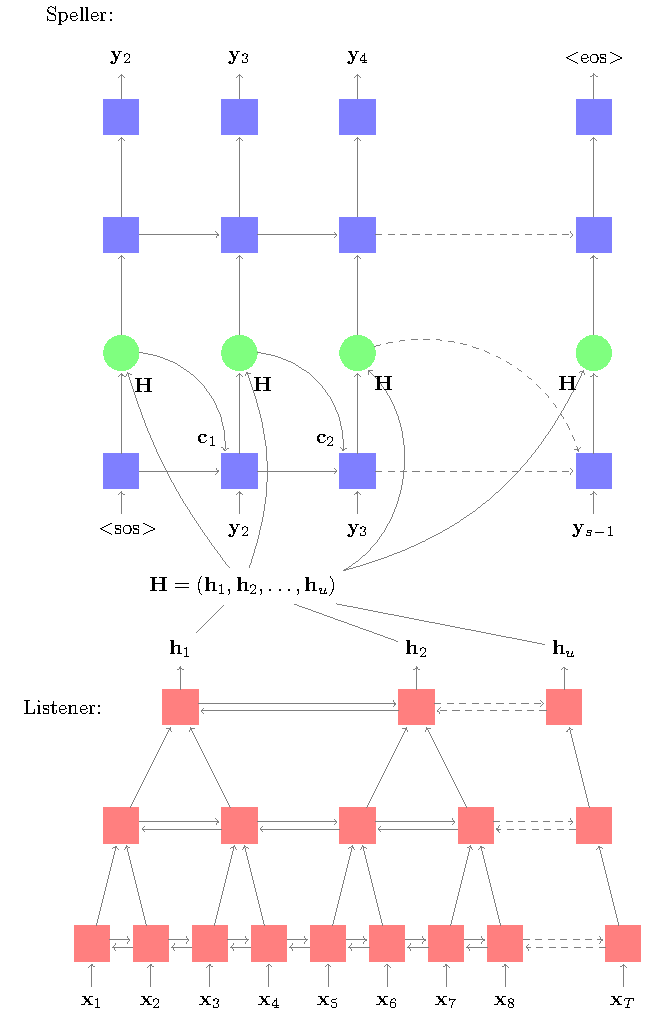
\includegraphics[height=6.5 cm]{../tikz/lasArcBottomUp}};
		    %\draw[red,ultra thick,rounded corners] (0.0,0.0) rectangle (5.0,2.5);
		\end{tikzpicture}
		\caption{Listener and speller.}
	\end{figure}
\end{frame}

\begin{frame}{The LAS-Equations}
Attend and spell cell computations:
\begin{align}
	 \mathbf{s}_i &= \text{RNN}(\mathbf{s}_{i-1}, \mathbf{y}_{i-1}, \mathbf{c}_{i-1}), \\
	 \mathbf{c}_i &= \text{AttentionContext}(\mathbf{s}_i,\mathbf{H}), \\
	  P(\mathbf{y}_i|\mathbf{x}, \mathbf{y}_{<i}) &= \text{CharacterDistribution}(\mathbf{s}_i,\textbf{c}_i).
\end{align}

AttentionContext computations:
\begin{align}
	e_{i,u} = \phi(\mathbf{s}_i)^T \psi(\mathbf{h_u}), \\
	\alpha_{i,u} = \frac{ \exp(e_{i,u})}{ \sum\limits_{u} \exp(e_{i,u})}, \\
	\label{eq:alphas}
	\mathbf{c}_i = \sum\limits_{u} \alpha_{i,u} \mathbf{h}_u.
\end{align}
\end{frame}

\section{Implementation}


\begin{frame}[fragile]
\frametitle{Major obstacles}
\begin{itemize}

\item Attend and spell cell
\item Decoding loop logic
	\begin{itemize}
	\item greedy decoding
		\begin{itemize}
		\item works with multiple utterances
		\end{itemize}
	\item beam search
		\begin{itemize}
		\item multiple hypotheses
		\item keeps track of hypotheses' probabilities, sequence elements, states, status (done?) and sequence lengths
		\end{itemize}
	\end{itemize}
\item Efficiency
\end{itemize}
\end{frame}

\begin{frame}{Attend and spell cell layout}
	\begin{figure}
	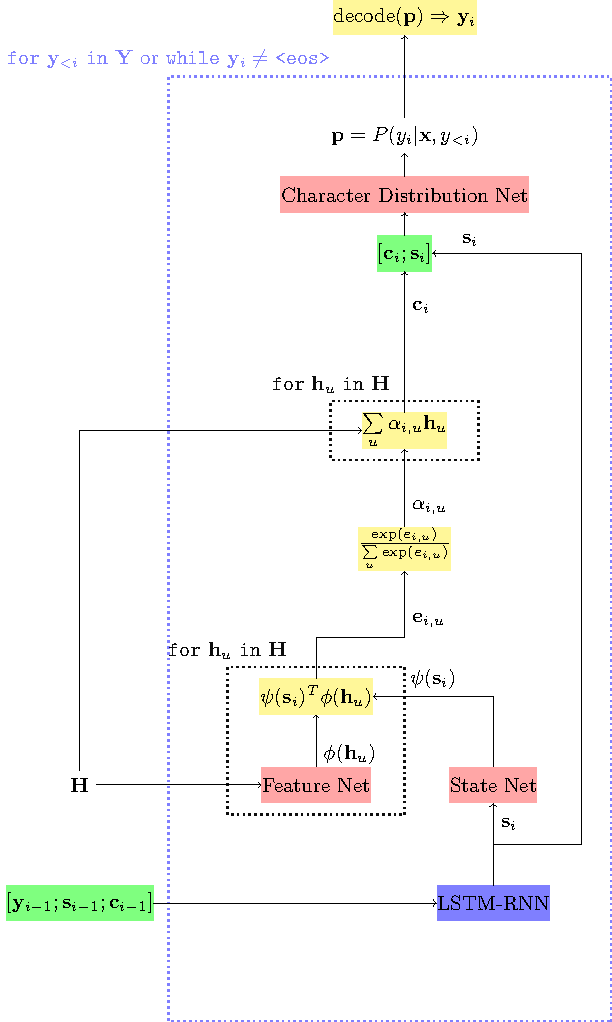
\includegraphics[height=6.5 cm]{../tikz/asCellType1}
	\caption{Attend and spell cell flow chart.}
	\end{figure}
\end{frame}

\begin{frame}{Efficency improvements}
	\begin{itemize}
		\item Evaluate the feature net output outside the attend and spell cell.
		\item Keep track of sequence lengths.
		\item Zero padding makes it possible to work with fixed size tensors.
		\item Sequence length information must be used to avoid processing the padding.
	\end{itemize}
\end{frame}

\begin{frame}{Dropout}
	\begin{figure}
		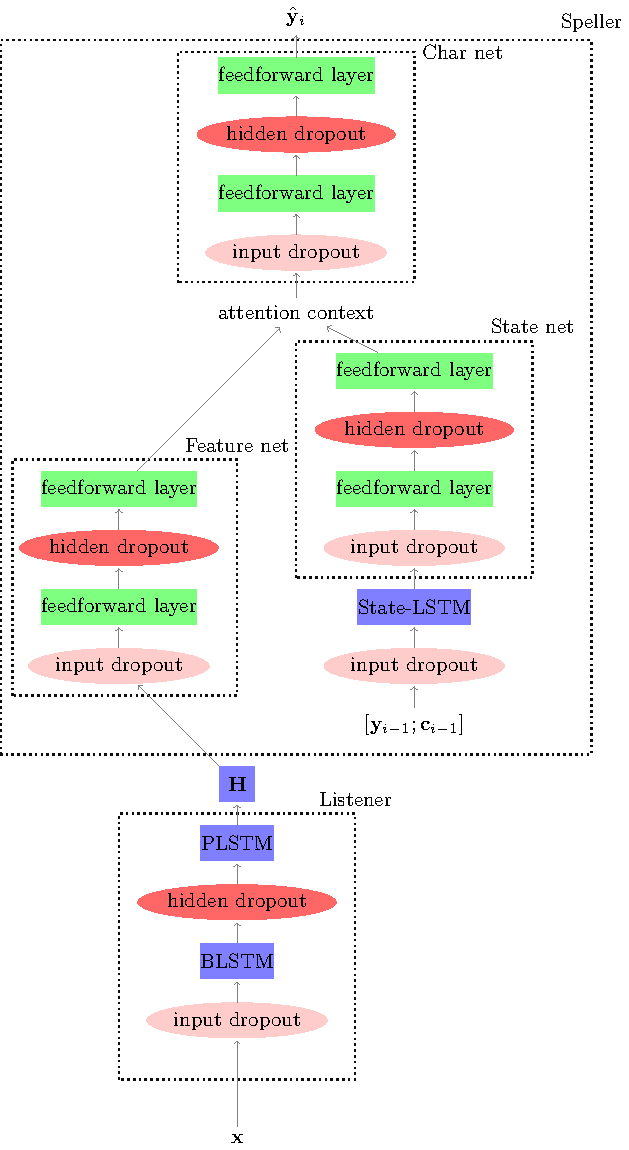
\includegraphics[height=6.5 cm]{../tikz/las_dropout}
		\caption{Input dropout - light red. Hidden dropout - dark red.}
	\end{figure}
\end{frame}

\section{Results}

\begin{frame}{Experimental settings}

\begin{itemize}
	\item TIMIT Speech corpus.
	\item learning rate: 0.001.
	\item batch\_size: 16 utterances, Training set total 3696.
	\item validation set size: 4 utterances.
	\item test set size: 192 utterances.
	\item validation every 20 weight updates.
\end{itemize}

\end{frame}


\begin{frame}{Greedy Decoding}
	\begin{figure}
	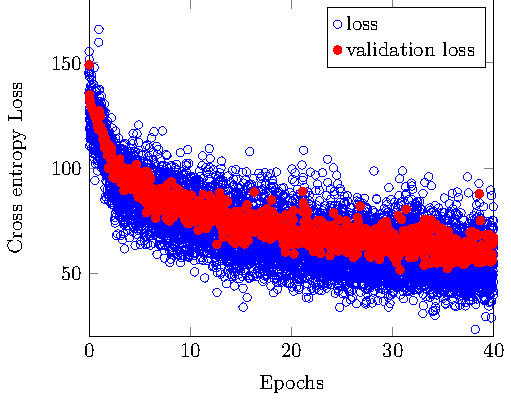
\includegraphics[width=0.49\linewidth]{../tikz/LAS_no_reg_e40_p07_loss}
	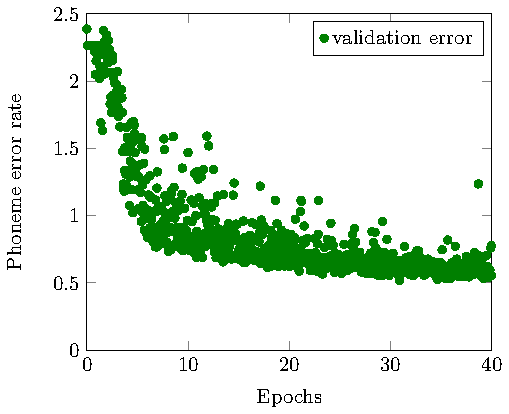
\includegraphics[width=0.49\linewidth]{../tikz/LAS_no_reg_e40_p07_error}
	\caption{The training progress shown for the full las architecture with greedy decoding, over 40 epochs, network output reuse probability 0.7 and input noise standard deviation 0.65.}
	\label{fig:lasGreedy}
	\end{figure}
\end{frame}

\begin{frame}{Alignment plots}
	\begin{figure}
	\centering
	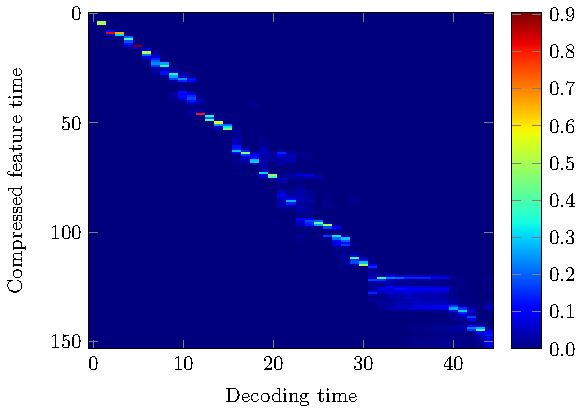
\includegraphics[width=0.49\linewidth]{../tikz/alpha}
	
\includegraphics[width=0.42\linewidth]{../tikz/align}
	\caption{Plot of the alignment vectors computed by the network for all 45 labels assigned to timit utterance \texttt{fmld0\_sx295} (left), and alignments assigned by a human listener (right).}
	\label{fig:fullAttention}
	\end{figure}
\end{frame}

\begin{frame}{Alignment plots}
	\begin{block}{Target labels}
		\begin{semiverbatim}
		<sos>  sil  ih  f  sil  k  eh  r  l  sil  k  ah  m  z
		       sil  t  ah  m  aa  r  ah  hh  ae  v  er  r  ey
		       n  jh  f  er  m  iy  dx  iy  ng  ih
		       sil  t  uw  sil
		<eos>
		\end{semiverbatim}
	\end{block}

	\begin{figure}
	\centering
	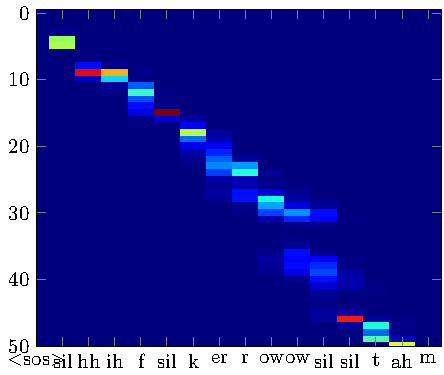
\includegraphics[height=0.26\linewidth]{../tikz/alphaZoom}
	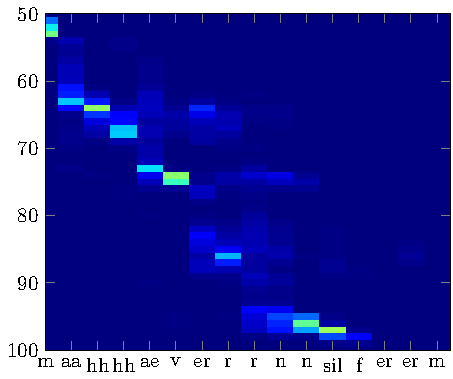
\includegraphics[height=0.26\linewidth]{../tikz/alphaZoom2}
	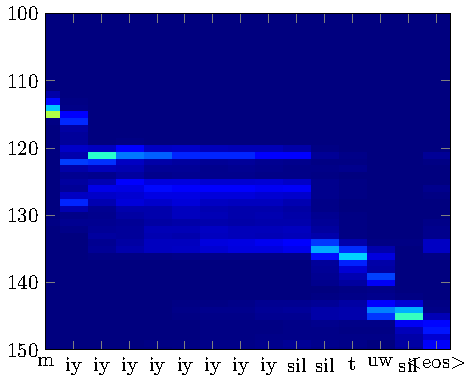
\includegraphics[height=0.26\linewidth]{../tikz/alphaZoom3}
	\caption{Attention weights $\alpha$ and network output.}
	\label{fig:attention3}
	\end{figure}
\end{frame}

\begin{frame}
	\begin{figure}
	\centering
	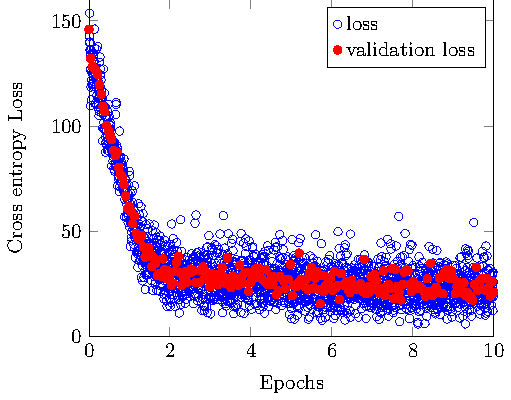
\includegraphics[width=0.24\linewidth]{../tikz/LAS_no_reg_e10_p02_loss}
	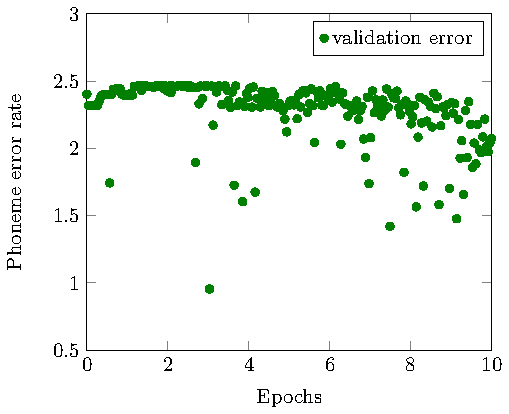
\includegraphics[width=0.24\linewidth]{../tikz/LAS_no_reg_e10_p02_error}
	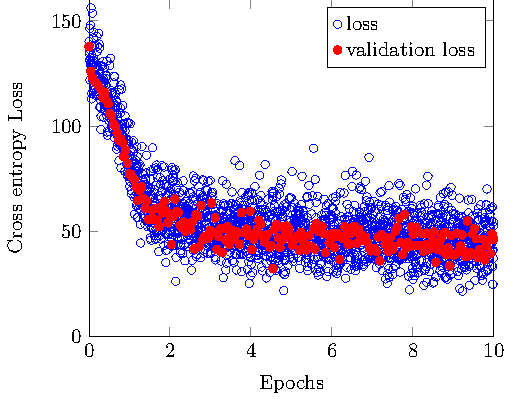
\includegraphics[width=0.24\linewidth]{../tikz/LAS_no_reg_e10_p04_loss}
	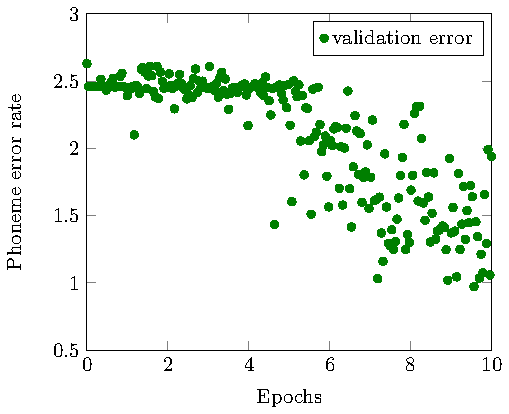
\includegraphics[width=0.24\linewidth]{../tikz/LAS_no_reg_e10_p04_error}
	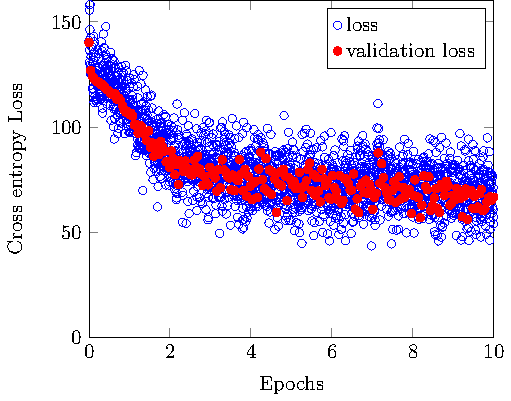
\includegraphics[width=0.24\linewidth]{../tikz/LAS_no_reg_e10_p06_loss}
	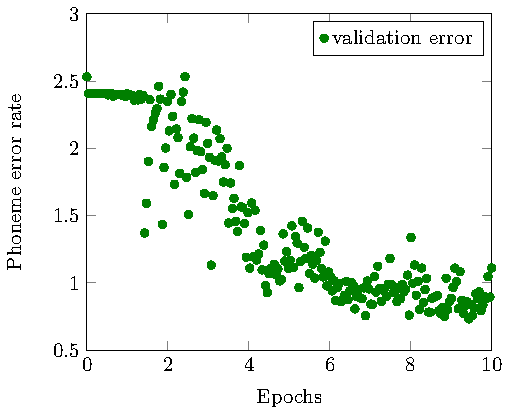
\includegraphics[width=0.24\linewidth]{../tikz/LAS_no_reg_e10_p06_error}
	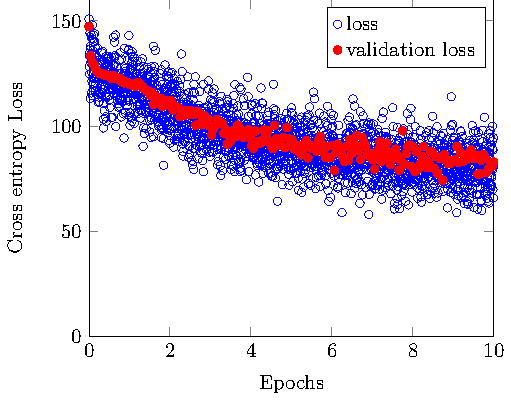
\includegraphics[width=0.24\linewidth]{../tikz/LAS_no_reg_e10_p08_loss}
	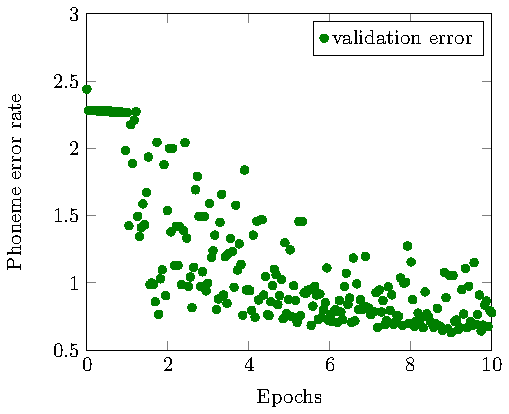
\includegraphics[width=0.24\linewidth]{../tikz/LAS_no_reg_e10_p08_error}
	\caption{Repetitions of the same experiment with increasing network output reuse probabilities $0.2, 0.4, 0.6, 0.8$, one experiment per row.}
	\label{fig:lasGreedy2468}
	\end{figure}
\end{frame}

\begin{frame}{Dropout las with beam search}
	\begin{figure}
	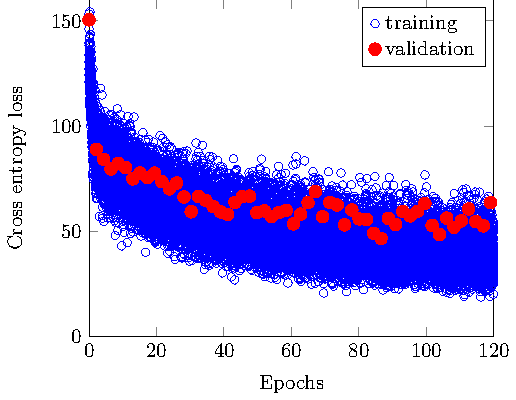
\includegraphics[width=0.49\textwidth]{../tikz/LAS_dropout0805_in00_p06_e120_double_loss}
	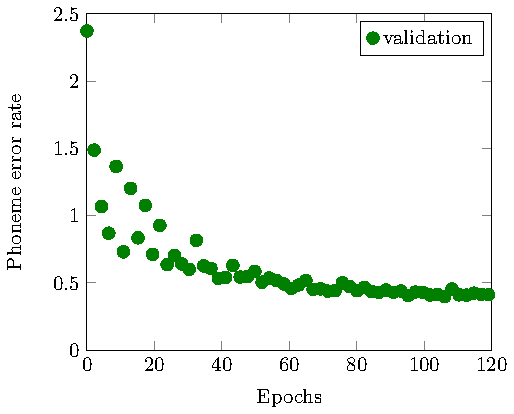
\includegraphics[width=0.49\textwidth]{../tikz/LAS_dropout0805_in00_p06_e120_double_error}
	\caption{Dropout las results.}
	\end{figure}
\end{frame}

\section{Conclusion}
\begin{frame}{Conclusion}

\begin{table}
\adjustbox{max height=\dimexpr\textheight-5.5cm\relax,
           max width=\textwidth}{
\begin{tabular}{ |l c |c c| c c c c| c| r| } \hline
\multicolumn{2}{|c|}{Experiment}  & \multicolumn{2}{|c|}{listener}  & \multicolumn{4}{|c|}{speller}       & epochs & error  \\ \hline
name 		   & 		reg			   	& dim  & layers			   	& dim   & net & layers	& $p$ reuse	  &  	   &        \\ \hline
BLSTM-CTC    & $\sigma_i=.65$          & 64   & 2	  			    & -	  	& -   & -	    & - 		  & 10     & 29\%   \\
Listener-CTC & $\sigma_i=.65$          & 64   & 2	                & -	    & -	  & -	    & -           & 10     & 26.8\% \\ \hline
Greedy-LAS   & $\sigma_i=.65$          & 64   & 2	                & 128   & 64   & 1,2	    & .7         & 40     & 55\%   \\
Greedy-LAS   & $\sigma_i=.65$          & 64   & 2	                & 128   & 64   & 1,2	    & .5         & 40     & 54\%   \\
Big-Beam-LAS   & $p_i=.8$,$p_h=.6$     & 128  & 2	                & 256   & 128  & 1,2	    & .6         & 40     & 45\%   \\ \hline
\end{tabular}
}
\caption{Selected important experiment parameters and test set phoneme error rate.}
\end{table}

\end{frame}

\begin{frame}{Conclusion}
\begin{itemize}
	\item Some success with a reimplemented LAS-architecture.
	\item Independent validation of beam search and dropout code required.
	\item Ways to improve:
		\begin{itemize}
			\item tensorflow's default attention mechanism.
			\item run larger networks.
			\item try other optimization parameters (learning rate, decay, \dots)
		\end{itemize}
\end{itemize}
\end{frame}


\section{Questions}
\begin{frame}{Questions}
	Thank's for your attention. Questions? \\
	Now, or later \texttt{moritz@wolter.tech}.
\end{frame}


\end{document}
